\section{总体结构}
\begin{frame}{智能体总体结构图}
    \centering
    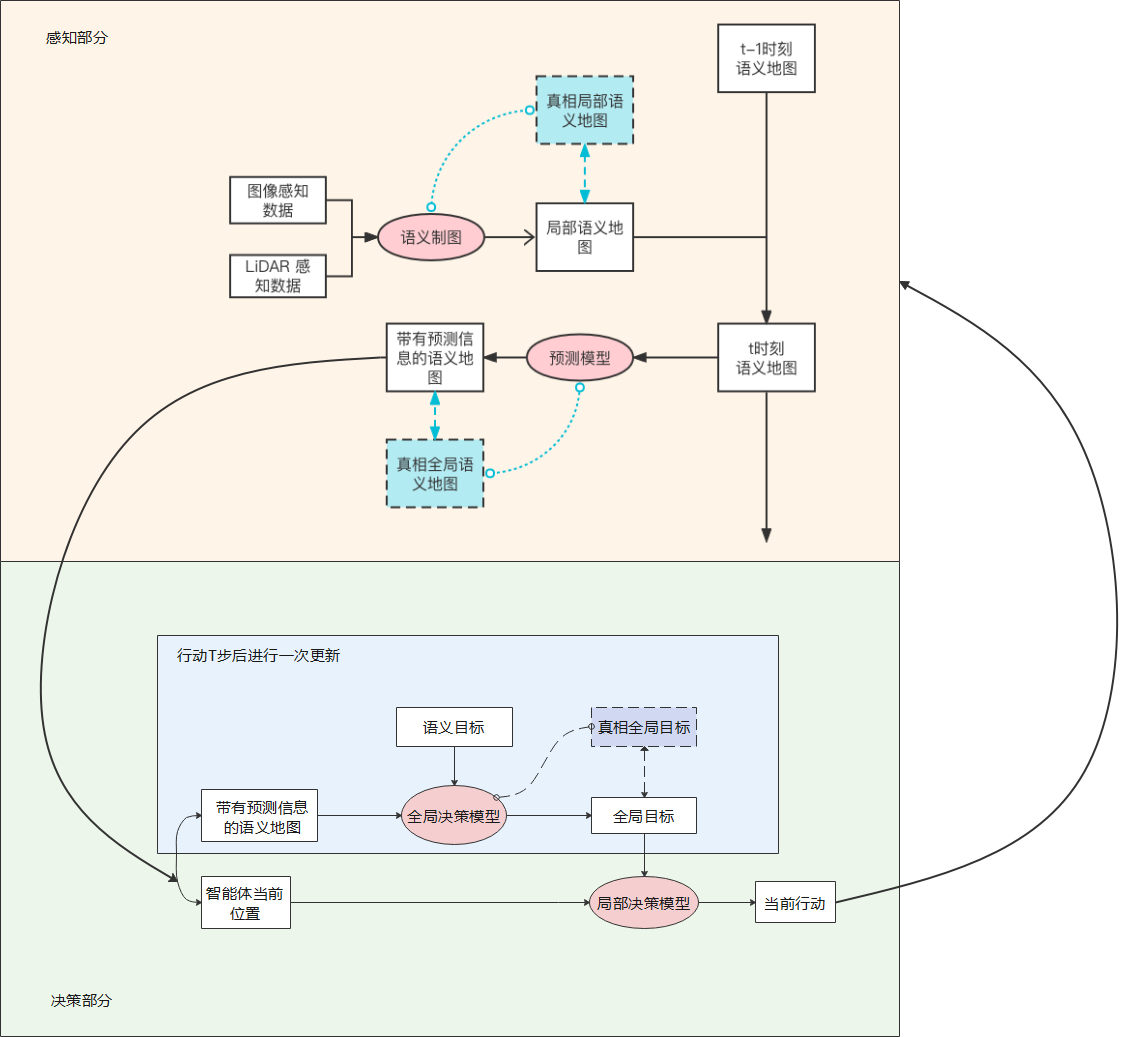
\includegraphics[width=8cm]{assets/integration.png}
    \note{
        图示是将两部分内容进行交互的整体图。
        \begin{itemize}
            \item 在每一步,感知输出的预测语义地图被决策部分接收,决策部分做出动作;
            \item 移动后感知部分将接收新的图像并产生新的预测语义地图,以此迭代。
            \item 以上过程在每一步都会执行,但全局目标的选择是粗粒度时间的,经历一定的步数才进行更新。
        \end{itemize}
    }
\end{frame}